\documentclass[crop,tikz]{standalone}
\usepackage{tikz}
\usepackage{sfmath}
\renewcommand{\familydefault}{\sfdefault}
\usepackage{pgfplots}
\usepgfplotslibrary{colorbrewer,patchplots}
\pgfplotsset{compat=1.18}
\renewcommand{\vec}{\mathbf}
\begin{document}
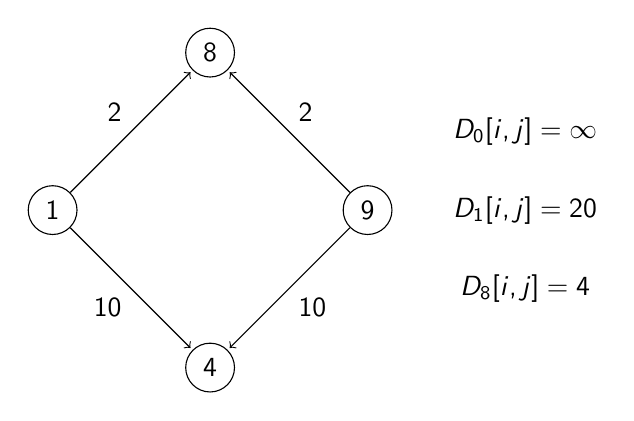
\begin{tikzpicture}[shorten >=1pt,->, vertex/.style = {draw, circle}]
    \node[vertex] (V1) at (-2, 0) {1};
    \node[vertex] (V8) at (0, 2) {8};
    \node[vertex] (V9) at (2, 0) {9};
    \node[vertex] (V4) at (0, -2) {4};

    \draw (V1) -- node[above left] {2} (V8);
    \draw (V9) -- node[above right] {2} (V8);
    \draw (V1) -- node[below left] {10} (V4);
    \draw (V9) -- node[below right] {10} (V4);

    \node at (4, 1) {$D_0[i,j] = \infty$};
    \node at (4, 0) {$D_1[i,j] = 20$};
    \node at (4, -1) {$D_8[i,j] = 4$};
\end{tikzpicture}
\end{document}